%% ENSF 612 Project Proposal (Milestone 1): DupHunter
\documentclass[11pt,a4paper]{article}

\usepackage[left=2cm,right=2cm,top=1.4cm,bottom=1.6cm]{geometry}
\usepackage[T1]{fontenc}
\usepackage{lmodern}
\usepackage{microtype}
\usepackage{booktabs}
\usepackage{tabularx}
\usepackage{array}
\usepackage[table]{xcolor}
\usepackage{tikz}
\usetikzlibrary{arrows.meta}
\usepackage{enumitem}
\usepackage{multicol}
\usepackage{float}
\setlist{nosep,leftmargin=*}
\usepackage[font=small,labelfont=bf,skip=3pt]{caption}
\usepackage{titlesec}
\titlespacing*{\section}{0pt}{6pt}{2pt}
\titleformat*{\section}{\large\bfseries}
\usepackage[colorlinks=true,linkcolor=blue!50!black,citecolor=blue!50!black,urlcolor=blue!50!black]{hyperref}

\setlength{\parskip}{4pt}
\setlength{\parindent}{0pt}
\setlength{\textfloatsep}{6pt}
\setlength{\intextsep}{6pt}
\newcolumntype{Y}{>{\raggedright\arraybackslash}X}
\newcommand{\g}{\cellcolor{blue!22}}
\newcommand{\ms}{\cellcolor{orange!45}}

\begin{document}

\begin{center}
  {\Large\bfseries ENSF~612 Project Proposal (Milestone~1)}\\[3pt]
  {\small Engineering Large-Scale Data Analytics Systems, Fall 2026\\[1pt]
  Instructor: Dr.~Ebrahim Karami\\[1pt]
  October 21, 2026}
\end{center}

%% ==========================================================================
\section{Project Title}
\textbf{DupHunter: Finding Duplicate Questions on Stack Overflow and Measuring
the Impact of AI}

%% ==========================================================================
\section{Group Members}
{\small
\begin{tabularx}{\textwidth}{@{}l Y@{}}
\toprule
\textbf{Name} & \textbf{Main role} \\
\midrule
Satyam Bhanot       & Data pipeline, Spark cluster setup, speed and scaling tests \\
Iesrat Jahan        & Duplicate detection (shingling, MinHash, LSH) \\
Md Jubayer Khan     & Popular tag combinations and expert ranking (SON, PageRank) \\
Navjot Singh Shienh & Stream counting and the AI-impact analysis \\
\bottomrule
\end{tabularx}}

%% ==========================================================================
\section{Problem Statement}

Stack Overflow is a website where programmers ask and answer questions. Many
new questions have already been asked before, just in different words. These
are called \emph{duplicates}. Today, volunteers find and close them by hand,
and many are missed.

We want to build a system that finds duplicate questions automatically. The
hard part is size. Stack Overflow has about 24 million questions. Comparing
every question with every other question would take years on one computer, so
we need methods that are built for large data and can run on many computers at
once.

We will also use the same data to look at a second question: how have AI tools
such as ChatGPT and GitHub Copilot changed Stack Overflow since they became
popular in 2022?

\textbf{Questions we want to answer:}
\begin{enumerate}[label=\textbf{Q\arabic*.},leftmargin=2.2em]
  \item Can we find most of the known duplicate questions without comparing
        every pair?
  \item How much faster does our system run when we add more computers?
  \item Which tags often appear together, and who are the top experts for each
        tag?
  \item How did the number of new questions and duplicates change after AI tools
        became popular, and which topics changed the most?
\end{enumerate}

\textbf{Expected outcome:} a working Spark pipeline that answers these four
questions, with measurements of both accuracy and speed.

%% ==========================================================================
\section{Motivation and Application}

Duplicate questions waste time. People wait for answers that already exist,
experts answer the same thing again, and volunteers spend hours searching. A
tool that finds duplicates could show a user an existing answer before they
even post. The same idea is used to remove repeated pages from web search
results and from AI training data.

The AI question is timely. A 2024 study found that Stack Overflow activity
dropped after ChatGPT was released~\cite{delrio2024}. We want to check this across all
questions, see which topics were hit hardest, and see whether duplicates
changed too.

This project fits ENSF~612 because the data is too large for simple methods.
It needs the course's tools for large data: MapReduce and Spark, similarity
search, frequent itemsets, stream algorithms, and PageRank~\cite{mmds}.

%% ==========================================================================
\section{Dataset}

\textbf{Source.} We will use the public Stack Exchange data dump on the Internet
Archive (\url{https://archive.org/details/stackexchange}). We checked it on
October 21. The newest release is from September 30, 2026~\cite{sedump}. It is
free to use under the CC~BY-SA~4.0 license.

\textbf{Size and format.} The Stack Overflow archive is a single 64.2\,GiB (68.9\,GB)
compressed file (\texttt{.7z}) covering July 2008 to September 2026. Inside, each
table is an XML file with one record per line. The dump has many tables, but we
only need the three in Table~\ref{tab:data}. Record counts are estimates from
older releases; we will update them after loading the data.

\begin{table}[H]
\centering
\caption{The data we will use.}
\label{tab:data}
\small
\begin{tabularx}{\textwidth}{@{}l l Y Y@{}}
\toprule
\textbf{Table} & \textbf{Records (approx.)} & \textbf{Fields we keep} & \textbf{What we use it for} \\
\midrule
Posts     & 60 million (24 million questions) & id, type, parent id, title, body, tags, date, author & Dates and tags for all questions; full text for a subset \\
PostLinks & 10 million & post id, related post id, link type & Known duplicate pairs (our answer key) \\
Users     & 22 million & id, reputation & Checking our expert ranking \\
Super User site & 1.4\,GB compressed & same tables & Testing our code \\
\bottomrule
\end{tabularx}
\end{table}

\textbf{How much data we will use.} Each question needs a different amount of
data, so we will only load what each part needs.
\begin{itemize}
  \item We keep only the columns listed above and skip every other table.
  \item Dates and tags for all 24 million questions are small. They are enough
        for the tag combinations (Q3) and the AI trend analysis (Q4).
  \item Duplicate detection (Q1) is the heavy part because it needs the full
        question text, and we need to run it many times to test different
        settings. We will run it on questions tagged \texttt{python} (roughly
        2 million; we will confirm the count), adding more tags if time allows.
        This is still a large-scale problem: 2 million questions make about
        2 trillion pairs. We only score duplicate pairs where both questions
        are in the subset.
  \item We will build and debug everything on the Super User site from the same
        dump. It has the same format but is about 50 times smaller.
\end{itemize}
The scaling tests (Q2) on growing parts of the subset will show how run time
grows, so we can estimate the cost of running on all 24 million questions.

\textbf{Data quality and limitations.}
\begin{itemize}
  \item Question text is stored as HTML, with code mixed into the writing.
  \item Deleted posts are missing, and deleted users show up as empty values.
  \item Not every duplicate was marked by volunteers, so our answer key is
        incomplete. Some of our matches may be real duplicates that were never
        marked, so our precision will be a lower bound.
  \item The most recent months are incomplete, because new questions may still
        be answered or closed.
  \item Working on one tag means our duplicate results may not hold for every
        topic.
\end{itemize}

\textbf{Preprocessing.} We will:
\begin{enumerate}
  \item Extract only the three tables we need and read them as a stream, so we
        never store hundreds of GB of unpacked XML.
  \item Keep only the needed columns and save them in Parquet format (a
        compressed table format that Spark reads quickly), split by year.
  \item For the subset, remove HTML tags and keep code blocks separate from the
        text.
  \item Break each subset question into short groups of words, called
        \emph{shingles}, for duplicate detection.
\end{enumerate}

%% ==========================================================================
\section{Proposed Methodology}

\begin{figure}[H]
\centering
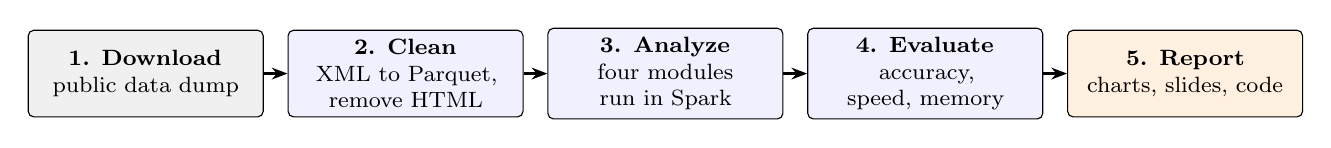
\begin{tikzpicture}[
  box/.style={draw, rounded corners=2pt, align=center, font=\footnotesize, text width=2.75cm, minimum height=1.1cm, fill=blue!6},
  arr/.style={-{Stealth[length=2mm]}, thick}
]
\node[box, fill=gray!12] (a) at (0,0)    {\textbf{1. Download}\\ public data dump};
\node[box]               (b) at (3.3,0)  {\textbf{2. Clean}\\ XML to Parquet, remove HTML};
\node[box]               (c) at (6.6,0)  {\textbf{3. Analyze}\\ four modules run in Spark};
\node[box]               (d) at (9.9,0)  {\textbf{4. Evaluate}\\ accuracy, speed, memory};
\node[box, fill=orange!12] (e) at (13.2,0) {\textbf{5. Report}\\ charts, slides, code};
\draw[arr] (a) -- (b); \draw[arr] (b) -- (c); \draw[arr] (c) -- (d); \draw[arr] (d) -- (e);
\end{tikzpicture}
\caption{Overview of the DupHunter pipeline.}
\label{fig:pipeline}
\end{figure}

Figure~\ref{fig:pipeline} shows the main steps. After cleaning, the data is
shared by four modules, one per team member:
\begin{itemize}
  \item \textbf{M1, Duplicate detection (Q1).} Turn each question into
        shingles, compress the shingles into a short MinHash
        \emph{signature}, then use LSH to put similar questions in the same
        bucket. We only compare questions that share a bucket, which avoids
        comparing every pair.
  \item \textbf{M2, Tags and experts (Q3).} Treat each question's tags as a
        ``basket'' and find tag combinations that often appear together. Build
        a graph of who answers whose questions and run PageRank for each tag to
        find the top experts.
  \item \textbf{M3, Stream counting (Q4).} Replay the posts in date order, as if
        they were arriving live, and use small-memory counters to track trending
        tags, active users, and duplicate rates over time.
  \item \textbf{M4, AI impact and system tests (Q2, Q4).} Compare monthly
        trends before and after AI tools became popular (June 2022 for Copilot,
        November 2022 for ChatGPT). Run speed and scaling tests on all modules.
\end{itemize}

\textbf{Running on many computers.} We will use Apache Spark (in
Python)~\cite{zaharia2012}, which follows the MapReduce model from the
course~\cite{dean2004}. Spark splits the data into chunks and processes them on
several computers at the same time. To avoid running out of memory, we will
process the LSH buckets in smaller batches and keep large intermediate results
on disk.

\textbf{How we will evaluate.}
\begin{itemize}
  \item \textbf{Accuracy (Q1):} Recall@K and Precision@K (how many known
        duplicates we find, and how many of our top K matches are correct), MAP
        (how high real duplicates rank), and reduction ratio (the share of pairs
        we never compare). We also check against exact results on a sample.
  \item \textbf{Correctness (Q3, Q4):} compare our own code to Spark's built-in
        versions and to exact counts.
  \item \textbf{Speed (Q2):} run time, memory use, and \emph{speedup}, meaning
        how many times faster the job runs on more computers. We will test
        1, 2, 4, and 8 workers and 10\%, 25\%, 50\%, and 100\% of the subset.
\end{itemize}

%% ==========================================================================
\section{Algorithms and Techniques}

We will write the main course algorithms ourselves and compare them with
ready-made Spark tools, so the report can clearly show which code is ours.

\begin{table}[H]
\centering
\caption{Algorithms we will build ourselves and what we compare them to.}
\label{tab:alg}
\small
\begin{tabularx}{\textwidth}{@{}l Y Y Y@{}}
\toprule
\textbf{Module} & \textbf{Course algorithms (our own code)} & \textbf{Compared with} & \textbf{Why we need it} \\
\midrule
M1 & Shingling, MinHash, LSH~\cite{broder1997,indyk1998} & Spark \texttt{MinHashLSH}; exact check on a sample & Find similar questions without comparing all pairs \\
M2 & SON frequent itemsets~\cite{son1995}; topic-sensitive PageRank~\cite{haveliwala2002} & Spark \texttt{FPGrowth}; GraphFrames PageRank & Popular tag combinations; top experts per tag \\
M3 & Count-Min Sketch~\cite{cormode2005}, DGIM~\cite{dgim2002}, Flajolet-Martin~\cite{fm1985} & Exact counts in Spark SQL & Count trends with very little memory \\
M4 & Before/after trend comparison; MapReduce-style Spark jobs & Same jobs on 1 vs.\ many workers & Measure AI impact and system speedup \\
\bottomrule
\end{tabularx}
\end{table}

%% ==========================================================================
\section{Expected Challenges}
{\small
\begin{tabularx}{\textwidth}{@{}p{6.3cm} Y@{}}
\toprule
\textbf{Challenge} & \textbf{How we plan to handle it} \\
\midrule
Duplicates written in very different words & Measure how often this happens; try a second similarity method if time allows \\
Missing duplicate labels & Treat precision as a lower bound; rely mainly on recall, which the missing labels do not affect \\
Very large file and limited memory & Read only the needed tables and columns; use a subset; test on Super User first \\
Some LSH buckets become huge (common phrases) & Limit bucket size and split large buckets \\
Choosing LSH settings (number of bands and rows) & Too few bands miss duplicates and too many give false matches; test several settings on Super User \\
Moving a lot of data between computers when grouping LSH buckets & Process the buckets in batches; measure data moved and time per step \\
PageRank on a graph with millions of users is slow & Keep the graph split the same way each round so little data moves; stop when the ranks stop changing \\
\bottomrule
\end{tabularx}}

%% ==========================================================================
\section{Expected Results}
We expect that:
\begin{itemize}
  \item LSH will find most known duplicates while skipping more than 99.9\% of
        all question pairs.
  \item Simple steps will speed up almost in line with the number of workers,
        while steps that move a lot of data between computers will speed up
        less.
  \item The small-memory counters will stay close to the exact counts while
        using far less memory.
  \item Common tag combinations will match real technology groups (for example,
        \texttt{python}, \texttt{pandas}, and \texttt{dataframe}), and our top
        experts will mostly be high-reputation users.
  \item New questions will drop after AI tools became popular, more in some
        topics than others.
\end{itemize}

%% ==========================================================================
\section{Initial Project Schedule}

The cleaned Super User data will be ready by October 24, so all four modules
can start in parallel; Stack Overflow (SO) runs follow.

\begin{table}[H]
\centering
\caption{Weekly plan (blue: main work; orange: milestone).}
\label{tab:plan}
\footnotesize
\setlength{\tabcolsep}{3pt}
\begin{tabularx}{\textwidth}{@{}Y l *{7}{>{\centering\arraybackslash}p{1.2cm}}}
\toprule
\textbf{Task (week starting)} & \textbf{Who} & \textbf{Oct 21} & \textbf{Oct 28} & \textbf{Nov 4} & \textbf{Nov 11} & \textbf{Nov 18} & \textbf{Nov 25} & \textbf{Dec 2} \\
\midrule
Clean data (Super User, then SO) & Satyam   & \ms Oct 24 & \g &  &  &  &  &  \\
Cluster setup and speed tests         & Satyam   &  & \g & \g &  & \g &  &  \\
Duplicate detection (M1)              & Iesrat   & \g & \g & \g & \g &  &  &  \\
Tags and experts (M2)                 & Jubayer  & \g & \g & \g & \g &  &  &  \\
Streams and AI impact (M3, M4) & Navjot  & \g & \g & \g & \g &  &  &  \\
Full runs and results                 & All      &  &  &  & \g & \ms Nov 21 &  &  \\
Presentation                          & All      &  &  &  &  & \g & \g &  \\
Final report and code                 & All      &  &  &  &  &  & \g & \ms Dec 4 \\
\bottomrule
\end{tabularx}
\end{table}

%% ==========================================================================
\section{References}
\vspace{-14pt}
\begin{multicols}{2}
{\footnotesize
\renewcommand{\section}[2]{}
\begin{thebibliography}{99}
\setlength{\itemsep}{0pt}
\setlength{\parskip}{0pt}
\bibitem{mmds} A.~Rajaraman and J.~D.~Ullman, \emph{Mining of Massive Datasets}. Cambridge University Press, 2011.
\bibitem{sedump} Stack Exchange, Inc., ``Stack Exchange Data Dump 2026-09-30,'' Internet Archive, \url{https://archive.org/details/stackexchange_20260930}.
\bibitem{delrio2024} R.~M.~del Rio-Chanona, N.~Laurentsyeva, and J.~Wachs, ``Large language models reduce public knowledge sharing on online Q\&A platforms,'' \emph{PNAS Nexus}, vol.~3, no.~9, 2024.
\bibitem{dean2004} J.~Dean and S.~Ghemawat, ``MapReduce: Simplified data processing on large clusters,'' in \emph{Proc. OSDI}, 2004.
\bibitem{zaharia2012} M.~Zaharia \emph{et al.}, ``Resilient distributed datasets: A fault-tolerant abstraction for in-memory cluster computing,'' in \emph{Proc. NSDI}, 2012.
\bibitem{broder1997} A.~Z.~Broder, ``On the resemblance and containment of documents,'' in \emph{Proc. Compression and Complexity of Sequences}, 1997.
\bibitem{indyk1998} P.~Indyk and R.~Motwani, ``Approximate nearest neighbors: Towards removing the curse of dimensionality,'' in \emph{Proc. ACM STOC}, 1998.
\bibitem{son1995} A.~Savasere, E.~Omiecinski, and S.~Navathe, ``An efficient algorithm for mining association rules in large databases,'' in \emph{Proc. VLDB}, 1995.
\bibitem{haveliwala2002} T.~H.~Haveliwala, ``Topic-sensitive PageRank,'' in \emph{Proc. WWW}, 2002.
\bibitem{cormode2005} G.~Cormode and S.~Muthukrishnan, ``An improved data stream summary: The count-min sketch and its applications,'' \emph{J. Algorithms}, vol.~55, no.~1, 2005.
\bibitem{dgim2002} M.~Datar, A.~Gionis, P.~Indyk, and R.~Motwani, ``Maintaining stream statistics over sliding windows,'' \emph{SIAM J. Comput.}, vol.~31, no.~6, 2002.
\bibitem{fm1985} P.~Flajolet and G.~N.~Martin, ``Probabilistic counting algorithms for data base applications,'' \emph{J. Comput. Syst. Sci.}, vol.~31, no.~2, 1985.
\end{thebibliography}}
\end{multicols}

\end{document}
